\documentclass[TAN.tex]{subfiles}
\begin{document}

\chapter{Funciones aritméticas}
\section{Divisibilidad}
Consideramos conocidos los conjuntos:
\[ \N = \{1,2,3,4,\dots\} \text{ números naturales}\]
\[ \Z = \{\dots,-3,-2,-1,0,1,2,3,\dots,\} \text{ números enteros}\]
y las operaciones de suma y producto definidas en ellos con las propiedades usuales. El conjunto $\Z$, dotado con las operaciones usuales es un \textbf{anillo conmutativo}. El anillo $\Z$ es un \textbf{dominio de integridad}, es decir, se cumple que si $ac=bc$ siendo $c \neq 0$ entonces $a=b$.

En $\Z$ tenemos definida una \textbf{relación de orden} $<$ tal que para todo $a$, $b$ y $c$ en $\Z$ se tiene
\begin{enumerate}
	\item $a < b \Rightarrow a+c < b+c$,
	\item Si $c > 0$ y $a < b \Rightarrow ac < bc$,
	\item O bien $a < b$ ó $b < a$ ó $a = b$.
\end{enumerate}
La relación de orden satisface la siguiente \textbf{propiedad de buen orden}: 
Si $A \subset \Z$ es no vacío y acotado inferiormente entonces existe $a \in A$ es es un mínimo de $A$.

A partir de estas hipótesis podemos desarrollar todas las propiedades que necesitamos.
En primer lugar definimos el conjunto de los números natural $\N = \{n \in \Z, n > 0\}$, los elementos positivos de $\Z$ de forma que
\[ \N = \{1,2,3,4,\dots\} \]

Supondremos deducidas las propiedades más simples.
Por ejemplo, $1 \in \N$, $\N$ es cerrado para la suma y el producto.
Si $a \in \Z$ es no nulo entonces $a$ ó $-a$ es un número natural.
Para todo $a \in \N$ el conjunto $\{x \in \N, x ≤ a\}$ es finito.

\begin{prop}[División]
Dados $a \in \Z$ y $b \in \N$ existen $q$ y $r$ tales que
\[ a = qb+r, \ 0 ≤ r < b \]
Los números $q$ y $r$ son únicos.
\end{prop}

\begin{nota}[Algoritmo de Euclides]
Para obtener el máximo común divisor de dos números naturales.
\end{nota}

\begin{defi}
Decimos que $a$ \textbf{divide a} $b$ si existe $q \in \Z$ tal que $qa=b$.
\end{defi}.
Escribimos entonces $a \mid b$ y en caso contrario $a \nmid b$.

\begin{prop}
Dados $a$ y $b$ en $\N$ existe el máximo común divisor de $a$ y $b$.
\end{prop}

Denotamos el máximo común divisor divisor de $a$ y $b$ por $(a,b)$.
Si $(a,b) = 1$ se deice que $a$ y $b$ son primos entre sí.
Escribiremos $a \perp b$ para denotar que $a$ y $b$ son primos entre sí.

\begin{prop}
Si $c \mid ab$ y $c$ es primos con $a$, entonces $c \mid b$.
\end{prop}

\begin{defi}
Un entero $p > 1$ se dice \textbf{primo} cuando no hhay divisores $d$ de $p$ que cumplan $1 < d < p$.
Si un entero $a > 1$ no es primo se dice que es \textbf{compuesto}.
\end{defi}

\begin{teorema}[Factorización única]
Cada número natural mayor que uno puede expresarse como el producto de numeros primos.
Esta expresión es única cuando los números primos que la forman se ordenan de menos a mayor.
\end{teorema}

Se le llama a veces Teorema fundamental de la Aritmética.


\section{Las funciones $d(n)$ y $σ(n)$}

\begin{defi}
Para cada número natural $n$ denotamos por $d(n)$ el número de los divisores de $n$ y por $σ(n)$ la suma de estos divisores.

Junto a éstas definimos para cada número real $α$ la función $σ_α$
\[ d(n) = \sum_{d\mid n} 1, \quad σ(n) = \sum_{d\mid n} d, \quad σ_α(n) = \sum_{d\mid n} d^α \]
\end{defi}

\begin{nota}
El exponente al que aparece elevada el número primo $p$ en la descomposición de $n$ se denota por $ν_p(n)$ (incluyendo el caso $ν_p(n)=0$ si el factor primo $p$ no aparece en la descomposición) de forma que para todo número natural $n$ se tiene
\[ n = \prod_p p^{ν_p(n)} \]
\end{nota}

\begin{prop}
Para todo $n = p_1^{a_1}p_2^{a_2}\cdots p_k^{a_k}$ se tiene
\[ d(n) = \prod_{j=1}^k (1+a_j) = \prod_p (1+ν_p(n)) \]
\end{prop}
\begin{dem}
La segunda igualdad es inmediata. Por otro lado, el número de factores que divide a $n = p_1^{a_1}p_2^{a_2}\cdots p_k^{a_k}$  partir de su descomposición los obtenemos por combinatoria. Cada $p_i$ podemos tomar lo de $a_i+1$ formas (según el exponente $0,1,\dotsc,a_i$ que tomemos).
\end{dem}
\begin{coro}
Si $n \perp m$, entonces $d(mn) = d(m)d(n)$.
\end{coro}

Tenemos de este modo el primer ejemplo de un concepto importante.

\begin{defi}
Una función $f : \N \to \C$ es \textbf{multiplicativa} si $f(mn) = f(m)f(n)$ siempre que $n$ y $m$ sean primos entre sí.

Una función tal que $f(mn)=f(m)f(n)$ para todo $m$ y $n$ se dice que es \textbf{completamente multiplicativa}.
Este concepto tiene menos importancia pues hay muchas funciones interesantes que son multiplicativas y pocas que lo sean completamente multiplicativas.
\end{defi}

\begin{prop}
Si $n \perp m$ la aplicación
\begin{align*}
	\{ u \in \N : u \mid n\} \times \{v \in \N : v \mid m\} & \rightarrow \{ w \in \N : w \mid nm \}\\
	(u,v) & \mapsto uv
\end{align*}
es una biyección.
\end{prop}
\begin{dem}
Denotemos por $f$ dicha biyección. 
\begin{itemize} 
\item Veamos la inyectividad. Sean $(a,b),(a',b')$ tales que $f(a,b)=f(a',b')$ entonces tenemos que $a\mid n$, $b'\mid m$, $ab=a'b'$. Se tiene que $a\perp b'$, pues
$$
1=xm+ym = x\alpha a + y\beta b' = k_1 a + k_2 b'
$$
Por tanto, $a\mid a'b' \Rightarrow a\mid a'$. Análogamente tenemos que $a'\mid a$, por lo que son iguales, de donde se prueba que $b=b'$. 
\item Veamos la sobreyectividad. Es inmediato ver que si $n=\prod_{i=1}^k p_i ^{a_i}$, $m=\prod_{j=1}^r q_j^{b_j}$, con $p_i \neq q_j$ por ser coprimos, entonces cualquier divisor de $mn$ debe ser de la forma
$$
c = \prod_{i=1}^k p_i ^{a_i'}\prod_{j=1}^r q_j^{b_j'} \qquad a_i' \in \{0,\dotsc,a_i\} \quad b_j' \in \{0,\dotsc,b_j\}
$$
Luego tomamos como preimagen el par $(a,b) = (\prod_{i=1}^k p_i ^{a_i'},\prod_{j=1}^r q_j^{b_j'})$. Es claro que $(a,b) \in D(n)\times D(m)$.
\end{itemize}
\end{dem}
\begin{prop} Si $f$ y $g$ son multiplicativas la función $f * g$ definida por
\[ f * g (n) = \sum_{d\mid n} f(d)g(n/d) \]
es también multiplicativa
\end{prop}

\begin{dem}
\[ (f*g)(nm) = \sum_{c\mid nm}f(c)g\left(\frac{nm}{c}\right) = \sum_{a\mid n,b\mid m}f(ab)g\left(\frac{nm}{ab}\right) \]
Usando que $f$ y $g$ son multiplicativas:
\begin{align*}
	(f*g)(nm) & = \sum_{a\mid n,b\mid m} f(a)f(b)g(n/a)g(m/b)  = \sum_{a\mid n}f(a)g(n/a) \sum_{b\mid m}f(b)g(m/b) \\
	& = (f*g)(m) \cdot (f*g)(n)
\end{align*}
\QED
\end{dem}

La función $f * g$ se llama la \textbf{convolución} (de Dirichlet) de $f$ y $g$.
Aunque ahora mismo su definición pueda parecer extraña, veremos su justificación al estduiar las series de Dirichlet.
A continuación veremos varias consecuencias interesantes de la proposición anterior.

\begin{ejs}
Las funciones $d$, $σ$ y $σ_α$ son multiplicativas pues son convoluciones de funciones multiplicativas
\begin{enumerate}
\item $d(n) =\sum_{d\mid n} 1 = 1 \ast 1 (n)$
\item $\sigma(n)= \sum_{d\mid n} d = 1 \ast f (n)$, con $f(n)=n$.
\item $\sigma_\alpha (n) = \sum_{d\mid n} d^\alpha = 1 \ast f (n)$, con $f(n)=n^\alpha$.
\end{enumerate}
\end{ejs}

\begin{prop}
Si $n = p_1^{a_1} \cdot p_n^{a_n}$, entonces
\[ σ(n) = \prod_{j=1}^r \frac{p_j^{a_j+1}-1}{p_j-1} = \prod_p \frac{p^{ν_p(n)+1}-1}{p-1} \]
\end{prop}
\begin{dem}
Basta aplicar la fórmula de la suma geométrica y tener en cuenta que si $n=p_1^{a_1}\cdots p_k^{a_k}$ entonces
$$\sigma(n) = \sum_{d\mid n} d = \prod_{i=1}^k \sum_{j=0}^{a_i} p^j$$
\end{dem}
\begin{defi}
Se dice que un número natural $n$ es perfecto si es la suma de sus divisores propios, estos es, si $σ(n)=2n$.
\end{defi}

\begin{teorema}[Euclides, Euler]
Los números perfectos pares son los números de la forma $2^{p-1}(2^p-1)$, donde $p$ recorre los números primos tales que $(2^p-1)$ sea también primo.
\end{teorema}
\newpage
\begin{dem}
Supongamos que $2^p -1$ es primo, entonces
$$
\sigma(n) =\sigma (2^{p-1}(2^p-1)) = \sigma(2^{p-1})\sigma(2^p -1) = \frac{2^{p-1+1}-1}{2-1}(2^p-1+1) =2^p(2^p-1)
$$
Por lo que $n$ es perfecto. Recíprocamente, supongamos que $n$ es par y perfecto, por lo que $n=2^am$ con $a\geq 1$ con $m$ impar. Tenemos que
$$
\sigma(n)=\sigma(2^am) = \sigma(2^a)\sigma(m) =\frac{2^{a+1}-1}{2-1}\sigma(m)=(2^{a+1}-1)\sigma(m)
$$
Por ser perfecto, $(2^{a+1}-1)\sigma(m) = 2^{a+1}m$, luego
$$
\sigma(m)=\frac{[(2^{a+1}-1)+1]m}{2^{a+1}-1} = \frac{m + m(2^{a+1}-1)}{2^{a+1}-1} = m + \frac{m}{2^{a+1}-1}
$$
Por lo que $m$ tiene solo dos divisores, $1$ y $m$ y $\frac{m}{2^{a+1}-1}=1$, $m=2^{a+1}-1$. Finalmente, veamos que si $2^p -1$ es primo entonces $p$ es primo. Si no lo fuera, entonces $p=mn$ y 
$$
2^{mn}-1 = (2^n)^m - 1 = (2^n-1)(1+2^n + \dotsc + 2^{(m-1)n})
$$
Lo cuál es una contradicción con el hecho de que $2^a-1$ sea primo.
\QED
\end{dem}
No se conoce si existen infinitos números perfectos, ni tampoco si existe alguno impar.


\section{Las funciones $φ(n)$ de Euler y $μ(n)$ de Möbius}
\begin{defi}
Se denota por $φ(n)$ el cardinal del conjunto de números primos con $n$ y menores que $n$.
\[ φ(n) = \text{card}\{k \perp n : 1 ≤ k ≤ n\} \]
\end{defi}
\begin{prop}
Para todo $n\in \N$, $n>1$ se tiene que 
$$
\varphi(n)=\abs{\left(\Z/\Z n\right)^\ast}
$$
\end{prop}
\begin{dem}
Sea $n\in \N$ fijo. Sea $1\leq a \leq n$ con $a\perp n$, por , $\exists x,y \in \Z$ tales que $1=xa+yn$. Tomando clases en $\Z/\Z n$, $[a][x]+[n][y]=[1]$, pero $[n]=0$, por lo que $[a]$ es unidad.

Recíprocamente, sea $[a]\in\left(\Z/\Z n\right)^*$, entonces $\exists  [b]\in\left(\Z/\Z n\right)^*$ tal que $[a][b]=[ab]=1$ Por tanto, $n\mid ab-1$, es decir, $\exists c$ tal que $1 = ab-nc$, por lo que $a\perp c$. Por tanto
$$
\varphi(n)= \text{card}\{k \perp n : 1 ≤ k ≤ n\} = \abs{\left(\Z/\Z n\right)^\ast}$$
\end{dem}
\newpage
\begin{prop}\mbox{}
\begin{enumerate}[(a)]
	\item La función φ es multiplicativa
	\item $φ(n) = n \displaystyle\prod_{p\mid n} \left(1-\dfrac{1}{p}\right)$
\end{enumerate}
\end{prop}

\begin{dem}
\begin{enumerate}[(a)]
\item Sean $m,n$ coprimos, entonces sabemos que 
$$
\Z/\Z nm \cong \Z/\Z n \times \Z/\Z m \Rightarrow \varphi(mn)= |(\Z/\Z nm)^*| = |(\Z/\Z n)^*||(\Z/\Z m)^*| = \varphi(n)\varphi(m)
$$

\item Usando que $φ$ es multiplicativa:
\[ φ(p^a) = p^a - p^{a-1} = p^a(1-1/p) \]
Sea $n = p_1^{a_1}\cdots p_k^{a_k}$:
\[ φ(n) = φ(p_1^{a_1})\cdots φ(p_k^{a_k}) = p_1^{a_1}(1-1/p_1)\cdots p_k^{a_k}(1-1/p_k) = n \prod_{p\mid n} \left(1-\dfrac{1}{p}\right)\]
\end{enumerate}
\QED
\end{dem}

\begin{teorema}[Teorema de Euler]
Si $a \perp n$ entonces $a^{φ(n)} \equiv 1 \pmod n$.
\end{teorema}
\begin{dem}
Sea $[a]\in {\left(\Z/\Z n\right)^\ast}$, Entonces ${\left(\Z/\Z n\right)^\ast} = [a]{\left(\Z/\Z n\right)^\ast}$, luego el producto de todos los elementos de cada conjunto debe coincidir
$$
[a][x_1]\cdots[a][x_{\varphi(n)}] = [a]^{\varphi(n)}\prod_{i=1}^{\varphi(n)} [x_i] = \prod_{i=1}^{\varphi(n)} [x_i] \Rightarrow [a]^{\varphi(n)} = 1
$$
\end{dem}
\begin{prop}
Para todo $n \in \N$ se tiene $\displaystyle\sum_{d\mid n} φ(d) = n$.
\end{prop}

\begin{dem}
Sea $f(n) = \sum_{d\mid n} φ(d)$ y $g(n) = n$. Sea $h(n) = 1$. Obsérvese que $f = φ * h$. Como $φ$ y $h$ son multiplicativas, $f$ es multiplicativa. Como $g$ también es mulitplicativa, para probar que $f = g$ basta ver que $f(p^a)=g(p^a)$ para un $p$ primo y $a ≥ 1$.

\[ f(p^a) = \sum_{b\mid p^a} φ(b) = \sum_{k=0}^a φ(p^k) = 1+(p-1)+(p²-p)+\cdots+(p^a-p^{a-1}) = p^a = g(p^a) \]
\qed

Como demostración alternativa:
\begin{align*}
n&= \left|\left\{\frac{a}{n} \mid 1 ≤ a ≤ n\right\}\right|
= \left|\bigcup_{b\mid n} \left\{\frac{a}{b} \mid 1≤a≤b, a \perp b\right\}\right|\\
&=\sum_{b\mid n} \left|\left\{\frac{a}{b} \mid 1 ≤ a ≤ b, a \perp b\right\}\right|
= \sum_{b\mid n} φ(b) 
\end{align*} \QED
\end{dem}

A continuación definimos la función de Möbius. Jugará un papel destacado en el curso y seguro que Möbius la consideraba tan importante como su famosa banda.

\begin{defi}
Se define la función de Möbius $μ(n)$ del siguiente modo
\[ μ(n) = \begin{cases}
	1 &\text{ si }n=1\\
	(-1)^k &\text{ si }n\text{ es producto de }k\text{ primos diferentes},\\
	0 &\text{ si }n\text{ es divisible por un cuadrado }>1
\end{cases}\]
\end{defi}

\begin{prop} Se tienen las siguientes propiedades para la función de Möbius
\begin{enumerate}[(a)]
\item La función de Möbius $μ$ es multiplicativa.
\item Para todo $n$
\[ \sum_{a\mid n} μ(a) = \begin{cases}
	1 & \text{ si } n = 1\\
	0 & \text{ si } n > 1
\end{cases}\]
\end{enumerate} 
\begin{dem}Pasemos a probar las propiedades.
\begin{enumerate}[(a)]
\item Sean $n=p_1^{a_1}\cdots p_k^{a_k}$ y $m=q_1^{b_1}\cdots q_s^{a_s}$ coprimos, entonces es claro que $$\mu(mn)=(-1)^{k+s}=(-1)^k(-1)^s=\mu(n)\mu(s)$$ pues un primo $p$ que divida a $mn$ divide o bien a $n$ o bien a $m$.
\item Dado $\mu(n)$, el miembro izquierdo de la ecuación $\mu \ast 1$, también es multiplicativo. El miembro derecho también es una función multiplicativa (obvio), basta probarlo para los números de la forma $p^a$ con $p$ primo y $a\geq 0$. El caso $a=0$ es trivial, en otro caso
$$
\sum_{d \mid p^a} \mu (d) = \sum_{n=0}^a \mu(p^n) = \mu(1)+\mu(p)=0
$$
\end{enumerate}
\end{dem}
\end{prop}

Finalmente un resultado importante son las dos fórmulas de inversión de Möbius.
En la primera se usa una técnica interesante para cambiar variables en sumas respecto de divisores.

\begin{prop}[Primera fórmula de inversión de Möbius]
Sean $f$ y $g$ dos funciones aritméticas, son equivalentes:
\begin{enumerate}[(a)]
	\item $\forall n$, $g(n) = \sum_{a\mid n} f(a)$
	\item $\forall n$, $f(n) = \sum_{a\mid n}μ(a) g(n/a)$
\end{enumerate}
\end{prop}
\newpage
\begin{dem}\mbox{}
\begin{itemize}
	\item Veamos que $(a) \Rightarrow (b)$
	\[
	\sum_{a\mid n} μ(a)g(n/a) = \sum_{a\mid n}μ(n/a)g(a) = \sum_{a\mid n}μ(a) \sum_{b\mid n/a} f(b) = \sum_{b\mid n}f(b)\left(\sum_{a\mid n/b} μ(a)\right) = f(n)
	\]
	\item Recíprocamente, veamos que  $(b) \Rightarrow (a)$
	\[
	\sum_{a\mid n}f(a) = \sum_{a\mid n} \sum_{b\mid a} μ(b)g(a/b) = \sum_{a\mid n}\sum_{b\mid a} μ(a/b)g(b) = \sum_{b\mid n}g(b)\left(\sum_{b\mid a\mid n}μ(a/b)\right) = g(n)
	\]
\end{itemize}
Veamos una demostración alternativa usando que $(1\ast \mu)$ es el elemento neutro de la convolución.
\begin{itemize}
\item Veamos que $(a) \Rightarrow (b)$
	$$
	\mu \ast g = \mu \ast (1 \ast f) = (\mu \ast 1)\ast f= f
	$$
	\item Recíprocamente, veamos que  $(b) \Rightarrow (a)$
	\[
	f \ast 1 = (\mu \ast g) \ast 1 = (g\ast \mu) \ast 1 = g \ast (\mu \ast 1) = g
	\]
\end{itemize}
\end{dem}

\begin{prop}[Segunda fórmula de inversión de Möbius]
Sean $F$ y $G$ funciones definidas en $(0,+∞)$ tales que $F((0,\varepsilon))=0$, para cierto $\varepsilon > 0$. Son equivalentes:
\begin{enumerate}[(a)]
\item $F(x) = \sum_{n=1}^{∞} G(x/n)$.
\item $G(x) = \sum_{n=1}^{∞} μ(n) F(x/n)$.
\end{enumerate}
\begin{dem}
Vamos a probar que $(a)$ implica $(b)$, pues la otra es análoga.
$$
\sum_{n=1}^{∞} μ(n) F(x/n) = \sum_{n=1}^{∞} μ(n) \sum_{m=1}^{∞} G(x/nm) = \sum_{r=1}^{∞} G(x/r) \sum_{d\mid r} \mu(d) = G(x)
$$
\end{dem}
\end{prop}

\begin{prop}[Segunda fórmula de inversión de Möbius]
Sean $F$ y $G$ funciones definidas en $[1,+∞)$. Son equivalentes:
\begin{enumerate}[(a)]
\item $F(x) = \sum_{n\leq x}^{∞} G(x/n)$.
\item $G(x) = \sum_{n\leq x}^{∞} μ(n) F(x/n)$.
\end{enumerate}
\begin{dem}
Vamos a probar que $(a)$ implica $(b)$, pues la otra es análoga.
$$
\sum_{n\leq x} μ(n) F(x/n) = \sum_{n\leq x} μ(n) \sum_{m\leq x/n} G(x/nm) = \sum_{r\leq x} G(x/r) \sum_{d\mid r} \mu(d) = G(x)
$$
\end{dem}
\end{prop}
\section{Series de Dirichlet}

Observemos como se comportan los monomios $x^n$ y $\dfrac{1}{n^s}$ al multiplicarlos
\[ x^n \cdot x^m = x^{n+m}, \qquad \frac{1}{n^s} \cdot \frac{1}{m^s} = \frac{1}{(mn)^s} \]
Los primeros generan las series de potencias, los segundos las series de Dirichet.
\[ \sum_{n=0}^{8} a_n x^n, \qquad \sum_{n=1}^{∞} \frac{a_n}{n^s} \]
Ahora sólo nos interesamos en su comportamiento formal.

A cada función aritmética $f(n)$ le podemos asociar, independientemente de su convergencia o no, una serie de Dirichlet
\[ \sum_{n=1}^{∞} \frac{f(n)}{n^s} \]
Lo que nos interesa sobre todo es como se multiplican estas series
\[ \left(\sum_{n=1}^{∞} \frac{f(n)}{n^s}\right)\left(\sum_{n=1}^{∞} \frac{g(n)}{n^s}\right) = \sum_{n=1}^{∞}\left(\sum_{d\mid n} f(d) g(n/d)\right) \frac{1}{n^s}\]

\begin{prop}
Dotado con el producto anterior y la suma usual, las series de Dirichlet forman un anillo.
\end{prop}
\begin{dem}
Las propiedades de anillo son triviales, pero hacemos la consideración de que cada serie de Dirichlet que converge en un punto $s$ verifica que
$$\sum_{n=1}^{∞} \frac{a_n}{n^s} \qquad s = \sigma + ri
$$
$|a_n|$ puede acotarse por
$$
|a_n| \leq C|n^s|=C|e^{s\log n}|= C|e^{\sigma \log n}| = Cn^\sigma
$$
\end{dem}
\begin{prop}
Las series de Dirichlet
\[ ζ(s) = \sum_{n=1}^{∞} \frac{1}{n^s}, \text{ y } ζ(s)^{-1}=\sum_{n=1}^{∞} \frac{μ(n)}{n^s} \]
son inversas en el anillo de las series de Dirichlet.
\end{prop}

\begin{prop}
Se tienen las relaciones en el anillo de las series de Dirichlet
\[ ζ(s)^2 = \sum_{n=1}^{∞} \frac{d(n)}{n^s},\ ζ(s)ζ(s-1)=\sum_{n=1}^{∞} \frac{σ(n)}{n^s},\ \frac{ζ(s-1)}{ζ(s)} = \sum_{n=1}^{∞} \frac{φ(n)}{n^s} \]
\end{prop}
\begin{dem}
\[ \sum \frac{d(n)}{n^s} = \left(\sum \frac{1}{n^s}\right) \cdot \left(\sum \frac{1}{n^s}\right) = ζ(s)^2 \]

\[ \sum_{n=1}^\infty \frac{σ(n)}{n^s} = ζ(s) \sum_{n=1}^\infty \frac{n}{n^s} = ζ(s) \sum \frac{1}{n^{s-1}} = ζ(s)ζ(s-1) \]
\[ \sum_{n=1}^\infty \frac{\varphi(n)}{n^s} = \sum_{n=1}^\infty \frac{μ(n)}{n^s} \sum_{n=1}^\infty \frac{n}{n^s} = \frac{\zeta(s-1)}{\zeta(s)} \]

\end{dem}

\section{Convergencia de series de Dirichlet}
\begin{teorema}
Si la serie de Dirichlet $\sum_{n=1}^\infty \frac{a_n}{n^s}$ converge en un punto $s = s_0$, entonces converge uniformemente en el ángulo $Γ_α = \{s \in \C : Re(s) > Re(s_0), |arg(s-s_0)|< α\}$ para cada $0 < α ≤ \pi/2$.
\end{teorema}

\begin{dem}
Por traslación podemos suponer que $s_0=0$. Además, podemos redefinir la serie de forma que $\sum_{n=1}^\infty a_n n^{-s} = 0$, pero esto implica que $\sum_{n=1}^\infty a_n = 0$. Definimos $s_n = \sum_{k=1}^n a_k$. Entonces, para $n>m$:
\begin{align*}
\left|\sum_{k=1}^n\frac{a_k}{k^s}-\sum_{k=1}^m\frac{a_k}{k^s}\right| &= \left|\sum_{k=m+1}^n\frac{a_k}{k^s}\right| = \left|\frac{s_{m+1}-s_m}{(m+1)^s} + \frac{s_{m+2}-s_{m+1}}{(m+2)^s}+\dots+\frac{s_{n}-s_{n-1}}{n^s}\right|\\
&= \left|\frac{s_n}{n^s}-\frac{s_m}{(m+1)^s}+\sum_{k=m+1}^{n-1}s_k\left(\frac{1}{k^s}-\frac{1}{(k+1)^s}\right)\right|\\
& ≤ \frac{\varepsilon}{n^σ} + \frac{\varepsilon}{(m+1)^σ} + \sum_{k=m+1}^{n-1} \varepsilon \left|\frac{1}{k^s}-\frac{1}{(k+1)^s}\right|
\end{align*}

Usando que:
\[ \left|\frac{1}{k^s}-\frac{1}{(k+1)^s}\right| = \left|\int_k^{k+1}-st^{-s-1}dt\right|≤ \int_k^{k+1}\left|st^{-s-1}\right|dt ≤ |s|\int_k^{k+1}t^{-σ-1}dt ≤ \frac{|s|}{σ} \left(\frac{1}{k^σ}-\frac{1}{(k+1)^σ}\right)\]

y que $n^σ ≥ 1$ y $(m+1)^σ ≥ 1$:

\[ \left|\sum_{k=1}^n\frac{a_k}{k^s}-\sum_{k=1}^m\frac{a_k}{k^s}\right| ≤ 2\varepsilon + \varepsilon \sum_{k=m+1}^{n-1} \frac{|s|}{σ}\left(\frac{1}{k^σ}-\frac{1}{(k+1)^σ}\right) = 2\varepsilon+\varepsilon\frac{|s|}{σ}\left(\frac{1}{(m+1)^σ}-\frac{1}{n^σ}\right) ≤ 2\varepsilon+\varepsilon\frac{|s|}{σ} \]
Como $σ/|s| = \cos(θ)$ donde $θ = \arg(s) ≤ α$, $|s|/σ ≤ (\sin α)^{-1}$, luego:
\[ \left|\sum_{k=1}^n\frac{a_k}{k^s}-\sum_{k=1}^m\frac{a_k}{k^s}\right| ≤ \varepsilon\left(2+\frac{1}{\sin α}\right) \]
Por tanto, la serie converge uniformemente.
\end{dem}

\begin{coro}
Si una serie de Dirichlet converge en algún punto, existe $σ_0 \in [-\infty,\infty)$, tal que la serie de Dirichlet define una función analitica en el semiplano $Re(s) > σ_0$ y divirge para todo $Re(s) < σ_0$. Decimos que $σ_0$ es la abcisa de convergencia de la serie de Dirichlet.
\end{coro}
\begin{dem}
La prueba es inmediata. Si $\sum_{n=1}\frac{a_n}{n^s}$ converge en $s_0$, $\exists \sigma_0\in[-\infty,\infty)$ tal que $\sum_{n=1}\frac{a_n}{n^s}$ converge uniformemente en $\Gamma_\alpha$. Concretamente, $\sigma_0 = \Re(s_0)$. Por otro lado
$$
\sum_{k=1} \frac{a_k}{k^s} = \sum_{k=1}a_ke^{-s\log k}
$$
donde $a_ke^{-s\log k}$ es analítica. Por tanto, $\sum_{k=1}a_ke^{-s\log k} = f(s)$ es una función analítica por ser una suma de analíticas que conforme uniformemente.
\end{dem}
\begin{ej}
La serie de Dirichlet $\sum_{n=1}^\infty \frac{(-1)^n}{n^s}$ tiene una abcisa de convergencia en $σ_0=0$. Obsérvese que no converge absolutamente en $0<σ<1$. De hecho, hay una abcisa de convergencia absoluta en $σ_0=1$.
\end{ej}

\begin{prop} Sea $f(s) = \sum_{n=1}^\infty a_n/n^s$ una función definida por una serie de Dirichlet. La función $f(s)$ es idénticamente $0$ si y sólo si todos los coeficientes $a_n$ son nulos.
\end{prop}
\begin{dem}
Sea $a_N$ el primer coeficiente distinto de 0. Se tiene entonces que:
\[ -\frac{a_N}{N^s} = \sum_{n=N+1}^{∞} \frac{a_n}{n^s} \]
 Sabemos que $\exists \alpha$ tal que la $f(\alpha)$ converge uniformmente, por lo que $\exists C$ de forma que $\abs{a_n}\leq C n^{\alpha}$. Sea ahora $\sigma >\alpha+1$
\begin{align*}
 \left|-\frac{a_N}{N^σ}\right| &= \left|\sum_{n=N+1}^{∞} \frac{a_n}{n^σ}\right| ≤ \sum_{n=N+1}^{∞} \frac{|a_n|}{n^σ}≤ C \sum_{n=N+1}^{∞} \frac{1}{n^{σ-α}} \\
 &≤ C \int_N^{∞} t^{α-σ} dt = C \left.\frac{t^{α-σ+1}}{α-σ+1}\right|_N^{∞} = \frac{C}{σ-α-1} \frac{1}{N^{σ-α-1}}
\end{align*}
De donde se deduce que
\[ |a_N| ≤ N^σ \frac{c}{σ-α-1} \frac{1}{N^{σ-α-1}} = \frac{CN^{α+1}}{σ-α-1} \underset{\sigma\to \infty}{\longrightarrow} 0\]
\end{dem}

\begin{prop} Sea $f$ multiplicativa y la serie de Dirichlet $\sum_{n=1}^\infty \frac{f(n)}{n^s}$ con abcisa de convergencia absoluta en $σ_0$. Entonces:
\[ \sum_{n=1}^\infty \frac{f(n)}{n^s} = \lim_{x \to \infty} \prod_{p≤x} \left(1+\frac{f(p)}{p^s} + \frac{f(p^2)}{p^{2s}}+\cdots\right) = \prod_{p} \left(1+\frac{f(p)}{p^s} + \frac{f(p^2)}{p^{2s}}+\cdots\right) \]
La serie dentro del producto del segundo miembro converge por ser una subserie de la serie de Dirichlet donde converge absolutamente. 
\end{prop}

\begin{dem}
En primer lugar, tenemos convergencia absoluta pues
$$
\abs{\sum_{n=1}^\infty \frac{f(n)}{n^s}} \leq \sum_{n=1}^\infty \frac{|f(n)|}{n^\sigma}<\infty
$$
Por otra lado, usando que $f$ es multiplicativa
$$
\prod_{p\leq x}\left(1+\frac{f(p)}{p^s}+\frac{f(p^2)}{p^{2s}}+\cdots\right)=  \sum  \frac{f(p_1^{b_1})\cdots f(p_a^{b_a})}{p^{b_1s}\cdot p_a^{b_a s}}=\sum_{P^+(n)≤x} \frac{f(n)}{n^s} 
$$
Estudiamos ahora 
\begin{align*}
\abs{\sum_{n=1}\frac{f(n)}{n^s}- \sum_{P^+(n)≤x} \frac{f(n)}{n^s}}&= \abs{ \sum_{P^+(n)>x} \frac{f(n)}{n^s} } \leq \sum_{P^+(n)>x} \frac{|f(n)|}{n^\sigma} \leq \sum_{n>x} \frac{f(n)}{n^s}  \underset{x\to \infty}{\longrightarrow} 0
\end{align*}
Por ser el resto de una serie uniformemente convergente. Basta ahora hacer $x\to \infty$.
\end{dem}
\begin{coro}

Si $f$ es además completamente multiplicativa y $p_1,\dots,p_a$ son todos los primos menores que $x$:
\[ \sum_{n=1}^\infty \frac{f(n)}{n^s} = \prod_{p}\left(1-\frac{f(p)}{p^s}\right)^{-1} \]
\end{coro}
\begin{dem}
 Ahora, usando que $f$ es completamente multiplicativa $f(p^k)=f(p)^k$. Sumamos la serie geométrica y obtenemos los resultados trivialmente.
\end{dem}
\section{Crecimiento de funciones multiplicativas}
\begin{teorema}
Sea $f(n)$ una función multiplicativa. Si $\lim_{p^k \to +∞} f(p^k) = 0$, entonces
\[ \lim_{n\to +∞} f(n) = 0 \]
\end{teorema}
\begin{dem}
Sabemos que, por hipótesis, $A=\{p^k\mid \abs{f(p^k)}\geq 1\}$ es finito. Sea $M=\prod_{p^k\in A} \abs{f(p^k)}$. Sea $\varepsilon > 0$ definimos $B_\varepsilon=\{p^k\mid \abs{f(p^k)}\geq \varepsilon/M\}$, también finito. Sea $N_\varepsilon = \prod_{p^k\in B_\varepsilon}p^k$. Sabemos que $n>N_\varepsilon$ es de la forma $p_1^{k_1}\cdots p_r^{k_r}$. Por otro lado, si $\{p_1^{k_1},\dotsc, p_r^{k_r}\} \subset B_\varepsilon$ entonces
$$
n = \prod_{i=1}^rp_i^{k_i} \leq \prod_{p^k\in B_\varepsilon}p^k = N_\varepsilon
$$
Luego $\exists p^k \notin B_\varepsilon$ en la factorización de $n$. Tenemos por tanto
$$
\abs{f(n)}=\abs{\prod_{i=1}^r f(p_i^{k_i})} = \abs{f(p^k)} \prod_{p_i^{k_i}\in A} \abs{f(p_i^{k_i})}\prod_{p_i^{k_i}\notin A} \abs{f(p_i^{k_i})} \leq \frac{\varepsilon}{M}\cdot M \cdot 1 = \varepsilon
$$
\end{dem}
\begin{prop}
\[ d(n) = \mathcal{O}(n^δ) \]
para todo $δ > 0$.
\end{prop}
\begin{dem}
\[ \frac{d(p^k)}{p^{kδ}} =  \frac{1+k}{p^{kδ}} = \frac{1+\frac{\log p^k}{\log p}}{p^{kδ}} \leq \frac{1+\frac{\log p^k}{\log 2}}{p^{k\delta}}\overset{p^k \to \infty}{\longrightarrow}0\]
Deducimos el resultado del Teorema anterior.
\end{dem}

\begin{prop}
Para todo $\varepsilon > 0$ se tiene que
\[ \lim_{n \to +∞} φ(n)/n^{1+\varepsilon} =0, \quad \lim_{n \to +∞} φ(n)/n^{1-\varepsilon} = +∞ \]
\end{prop}
\begin{dem}
Usaremos el Teorema 1.6.1 y probaremos el primero, pues el otro es análogo.

$$
\frac{\varphi(p^k)}{p^{k(1+\varepsilon)}} = \frac{p^k(1-\frac{1}{p})}{p^{k(1+\varepsilon)}} = \frac{1-\frac{1}{p}}{p^{k\varepsilon}} \leq \frac{1}{p^{k\varepsilon}} \underset{p^k\to \infty}{\longrightarrow} 0
$$
\end{dem}
El \textbf{orden máximo} y el \textbf{orden mínimo} de una función aritmética $f(n)$ se definen como funciones monótonas crecientes $g(n)$ tales que
\[ \limsup_{n\to+∞} \frac{f(n)}{g(n)} = 1, \quad \text{respectivamente }\liminf_{n\to+∞}\frac{f(n)}{g(n)} = 1 \]
\begin{prop}
El orden mínimo de $\log d(n)$ es $\log 2$ y el orden máximo es
\[ \frac{\log 2 \log n}{\log \log n} \]
\end{prop}
\begin{dem}
El orden mínimo es claro, pues $d(n)\geq 2$ y se repite a lo largo de los infinitos primos. Vamos a demostrar el orden máximo. Vamos a ver que
\[ \limsup \frac{\log d(n)}{\frac{\log 2 \log n}{\log \log n}} = 1\]
Sabemos que $d(n)/n^{\varepsilon}\to 0$. Si $k=\min_{p\mid n} \nu_p(n)$, como $ \prod_{p^\alpha\geq 2} \frac{k+1}{p^{k\alpha}}  \to 1$ y que $e^x \geq x+1$, entonces
\begin{align*}
\frac{d(n)}{n^\alpha} &\leq \prod_{p\mid n} \frac{k+1}{p^{k\alpha}} = \prod_{p^\alpha\geq 2} \frac{k+1}{p^{k\alpha}}  \prod_{p^\alpha< 2} \frac{k+1}{p^{k\alpha}} {\leq }  \prod_{p^\alpha< 2} \frac{k+1}{p^{k\alpha}} \\
&\leq \prod_{p^\alpha< 2}1+ \frac{k}{p^{k\alpha}} \leq \prod_{p^\alpha< 2}1+ \frac{k}{\log p^{k\alpha}}\leq \prod_{p^\alpha< 2}1+ \frac{1}{\alpha\log p}\\
&\leq \prod_{p^\alpha< 2}e^{\frac{1}{\alpha\log p}} \leq  \prod_{p^\alpha< 2}e^{\frac{1}{\alpha\log 2}} \leq \exp\left\{\frac{\card{\{p\mid p^\alpha <2\}}}{\alpha\log 2}\right\}\\
&\leq \exp\left(\frac{2^{1/δ}}{δ\log 2}\right)
\end{align*}
Dado $\delta>0$, aplicando logaritmo a la expresión $\frac{d(n)}{n^δ} ≤ \exp\left(\frac{2^{1/δ}}{δ\log 2}\right)$.
\[
	\log d(n) ≤ δ\log n + \frac{2^{1/δ}}{δ\log 2}
\]
Sea $δ = (1+\varepsilon)\dfrac{\log 2}{\log \log n}$, entonces:
\[
	\log d(n) ≤ (1+\varepsilon) \frac{\log 2 \log n}{\log \log n} + \frac{(\log n)^{1/(1+\varepsilon)}}{(\log 2)^2} \frac{\log \log n}{1+\varepsilon} =: (1+\varepsilon)f(n) + g(n)
\]
Dividiendo por $f(n)$:
\[ 
	\frac{\log d(n)}{f(n)} ≤ 1 + \varepsilon + \frac{g(n)}{f(n)}
\]
Se observa además que $\dfrac{g(n)}{f(n)} \to 0$ si ${n \to ∞} $, luego:
\[ 
	\limsup \frac{\log d(n)}{f(n)} ≤ 1+\varepsilon
\]
Como esto se da para todo $\varepsilon$, se cumple que:
\[ 
	\limsup \frac{\log d(n)}{\frac{\log 2 \log n}{\log \log n}} ≤ 1
\]
Por otro lado, tomando $n(x) = \prod_{p≤x} p$, entonces:
\[ \log n = \sum_{p≤x} \log p = \theta(x) ≤ \sum_{p≤x} \log x = π(x) \log x \]
\[ d(n) = 2^{π(x)} \]
se llega a que:
\begin{align*}
\frac{\log d(n)}{\frac{\log 2 \log n}{\log \log n}} &= \frac{\log d(n) \log\log n}{\log 2 \log n} \geq \frac{\pi(x)\log 2 \log\log n}{\log 2 \log n} =  \frac{\pi(x) \log\log n}{\log n}\\
&=  \frac{\pi(x) \log\theta(x)}{\theta(x)} \geq \frac{\pi(x)\log \theta(x)}{\pi(x)\log x} \geq \frac{\log(Ax)}{\log x} \to 1
\end{align*}  
Luego:
\[
	\limsup \frac{\log d(n)}{\frac{\log 2 \log n}{\log \log n}} = 1 
\]
\end{dem}
\newpage
\section{Sumación parcial}
La idea básica que queremos desarrollar es la aproximación de una suma por una integral, y se puede plasmar en una figura.

\begin{teorema}[Comparación de una suma y una integral]
Sea $f : (0,+\infty) \to [0,+\infty)$ una función positiva y decreciente. Existe una constante $γ(f)$ tal que para todo $x>1$ se tiene
\[ \sum_{n≤x} f(n) = \int_1^x f(t)dt + γ(f) + \mathcal{O}(f(x)) \]
\end{teorema}
\begin{dem}
Tenemos $f$ positiva y decreciente. Vamos a estudiar la suma
$$
\sum_{n\leq x}f(n) = \sum_{n=1}^N f(n) \qquad N=\suelo{x}
$$
Se observa que la suma se aproxima al área bajo la curva $S\sim I = \int_1^x f(t)dt$. La diferencia $S-I$ es igual a 
$$S-I = \sum_{k=1} a_k < \infty$$ pues se observa que la suma de todos está contenido en un rectángulo de base $1$ y altura $f(1)$. Por tanto
$$
\gamma(f) = \sum_{k=1} a_k \leq f(1) \qquad S - I \sim \gamma(f) 
$$
La aproximación se da con un error $R(x)$ tal que $|R(x)|\leq f(x)$, por lo que
$$
\sum_{n\leq x} f(n) = \int_1^x f(t)dt + \gamma(f) + O(f(x))
$$
\QED
\end{dem}

\begin{teorema}
Existe una constante $γ$ tal que para todo $x>1$
\[ \sum_{n≤x} \frac{1}{n} = \log x + γ + \mathcal{O}\left(\frac{1}{x}\right) \]
\end{teorema}
La constante $γ$ se denomina constante de Euler, su valor aproximado es $γ \approx 0.577215663...$ Es un problema abierto decidir si es racional o irracional.

Clásicamente se llama sumación de Abel al proceso en que convertimos una suma $\sum_n a_n b_n$ mediante las sumas parciales $\sum_n a_n$. Esto es, definiendo $A_n = \sum_{j=1}^n a_j$ $ A_0 = 0$
la transformación es
\[ \sum_{j=1}^n a_j b_j = \sum_{j=1}^n (A_j-A_{j-1})b_j = \sum_{j=1}^{n-1} A_j(b_j-b_{j+1}) + A_n b_n \]
Este tipo de argumento es análogo al de la integración por partes. Si $A(x)=\int_a^x a(t)dt$
\[ \int_a^x a(t)f(t) dt = \int_a^x f(t) dA(t) = \left.f(t)A(t)\right|_a^x - \int_a^x A(t) df(t) = A(x)f(x) - \int_a^x A(t) df(t) \]
en el siguiente teorema lo extendemos al caso en que $A$ es una función de salto.

\begin{teorema}[Fórmula de Abel] Sea $(a_n)$ una sucesión de números complejos. Pongamos
\[ A(x) = \sum_{n≤x} a_n \quad (x > 0) \]
Sea $f(t)$ una función con derivada continua en $[1,x]$. Entonces tenemos
\[ \sum_{1≤n≤x} a_nf(n) = A(x)f(x)-\int_1^x A(t)f'(t)dt \]
\end{teorema}

\section{El orden medio de $d(n)$}
Como vemos, hemos tenido que pasar a $\log d(n)$ para poder determinar el orden máximo. El tomar logaritmos obviamente hace la función más manejable. Otra forma de resolver e problema es estudiar el \textbf{orden medio}, s llama así a una función $g(n)$ monótona y tal que
\[ f(1) + f(2) + \cdots + f(n) \sim g(1) + g(2) + \cdots + g(n) \]
\begin{teorema}[Dirichlet]
Cuando $x$ tiende a infinito, tenemos
\[ \sum_{n≤x} d(n) = x \log x + (2γ -1)x + \mathcal{O}(\sqrt{x}) \]
\end{teorema}

\begin{dem}
\[ \sum_{n≤x} d(n) = \sum_{n≤x}\sum_{a\mid n}1 =\sum_{a\leq x}\sum_{a\mid n \leq x} 1 = \sum_{a≤x}\suelo{ \frac{x}{a}} = \sum_{ab≤x} 1 \]
Consideramos el retículo $\mathcal{R}=\{(n,m) \mid  n \in \N,m \in \N, nm≤x\}$. Se tiene que $\sum_{ab≤x} 1 = \#\mathcal{R}$. Si particioneros $\mathcal{R}$ en los conjuntos: 
$$A=\{(n,m) \mid n \in \N,m \in \N, nm≤x, m≤\sqrt{x}\}$$
$$B=\{(n,m) \mid n \in \N,m \in \N, nm≤x, m>\sqrt{x}\}$$
$$C=\{(n,m) \mid n \in \N,m \in \N, n,m≤\sqrt{x}\}$$

\begin{figure}[htp!]
\centering
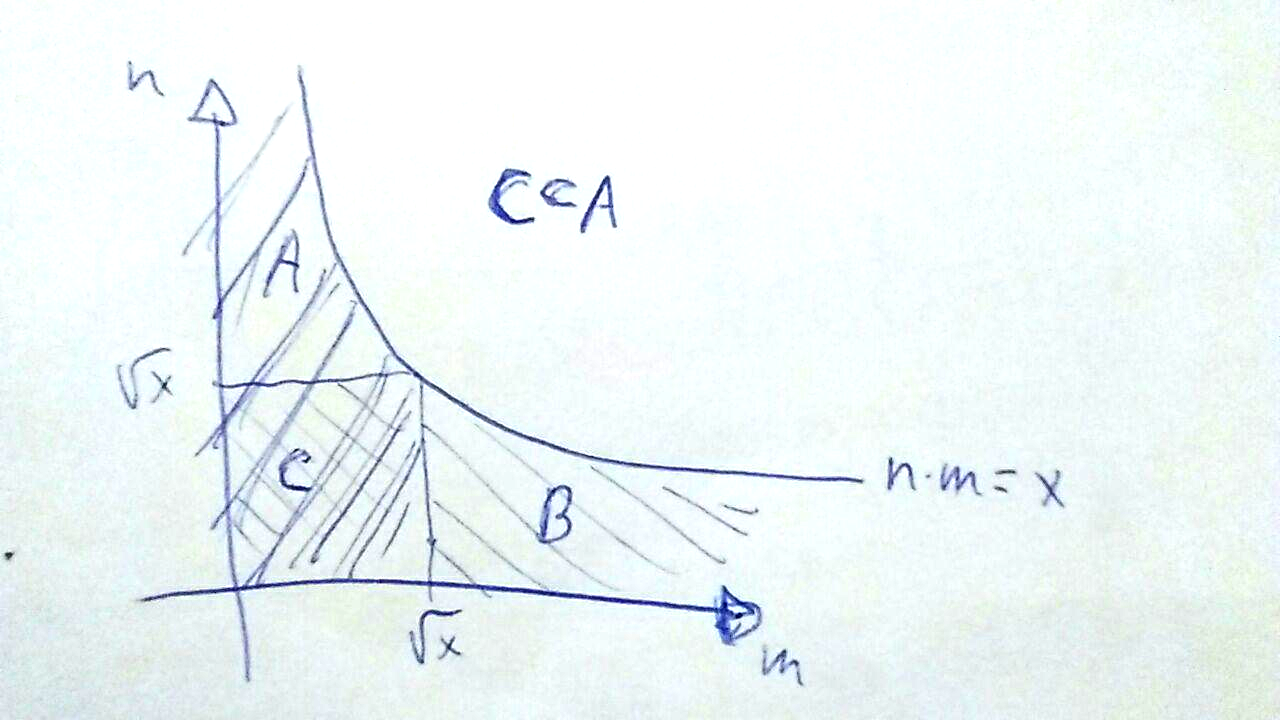
\includegraphics[width=260px]{images/hiperbola}
\end{figure}

Véase que $\#(A-C)=\#(B)$, luego $\#(R)=\#(A)+\#(B)-\#(C)=2\#(A)-\#(C)$.
Además, pues que $C$ es un cuadrado de lado $\sqrt{x}$, $\#(C)=\suelo{\sqrt{x}}^2$.
Se tiene que $\#A=\#B$, luego $\#\mathcal{R}=2\#A-\#C$. Además, pues que $C$ es un cuadrado de lado $\sqrt{x}$, $\#C=\suelo{\sqrt{x}}^2$.

\begin{align*}
	\sum_{ab≤x} 1 & = 2 \# A - \suelo{ \sqrt{x} }^2 = 2 \sum_{a≤\sqrt{x}} \suelo{ \frac{x}{a}} - \suelo{ \sqrt{x} }^2\\
	&= 2 \sum_{a≤x} \left(\frac{x}{a}-\left\{\frac{x}{a}\right\}\right) - (\sqrt{x}-\{\sqrt{x}\})^2 \\
	& = 2x \sum_{a ≤ \sqrt{x}} \frac{1}{a} + \mathcal{O}(\sqrt{x}) - (x-2\{\sqrt{x}\} \sqrt{x} + \{\sqrt{x}\}^2)  \\
	& = 2x(\log\sqrt{x} + γ + \mathcal{O}\left(\frac{1}{x}\right)) + \mathcal{O}(\sqrt{x}) -x+\mathcal{O}(\sqrt{x})+\mathcal{O}(1)\\
	&= x \log x + (2γ-1)x+\mathcal{O}(\sqrt{x})
\end{align*}
donde $\{x\} = x-\suelo{ x }$ y hemos usado que $-\sum_{a\leq x} \left\{\frac{x}{a}\right\} \leq \sqrt{x}$ es la parte fraccionaria de $x$. Luego $\sum_{n≤x} d(n) = x \log x + (2γ-1)x + \mathcal{O}(\sqrt{x})$.
\qed
\end{dem}


La técnica usada en la prueba se debe a Dirichlet y se denomina \textbf{método de la hipérbola}.

El término de error $\mathcal{O}(\sqrt{x})$ puede mejorarse. La determinación del ínfimo de los $θ$ tales que podamos substituir $\mathcal{O}(\sqrt{x})$ por $\mathcal{O}(x^{θ})$ en el teorema anterior, constituye un problema abierto que se onoce con el nombre de \textbf{problema del divisor de Dirichlet}. En 1915 Hardy y Landau probaron que $\inf θ ≥ 1/4$.

Por un método más simple podemos obtener el siguiente resultado.
\begin{teorema}
Para $x≥1$
\[ Φ(x) = \sum_{n≤x} φ(n) = \frac{3x^2}{π^2} + \mathcal{O}(x\log x) \]
\end{teorema}
\begin{dem}
\begin{align*}
	\sum_{n≤x} φ(n) & = \sum_{n≤x}\sum_{a\mid n} μ(a) \frac{n}{a} = \sum_{a≤x} \frac{μ(a)}{a}\left(\sum_{a\mid n≤x}n\right) =\sum_{a≤x} \frac{μ(a)}{a}\sum_{k=1}^{\suelo{x/a}} ka\\
	&= \frac{1}{2} \sum_{a≤x} μ(a)\left(\suelo{ \frac{x}{a}}^2 + \suelo{ \frac{x}{a}} \right)\\
	& = \frac{1}{2} \sum_{a≤x} μ(a) \left(\left(\frac{x}{a} - \left\{ \frac{x}{a}\right\} \right)^2 + \frac{x}{a}-\left\{\frac{x}{a}\right\}\right)\\
	& = \frac{1}{2} \sum_{a≤x} μ(a) \left(\frac{x^2}{a^2} - 2\left\{\frac{x}{a}\right\}\frac{x}{a} + \left\{\frac{x}{a}\right\}^2+\frac{x}{a}-\left\{\frac{x}{a}\right\}\right)\\
	&  = \frac{x^2}{2} \sum_{a≤x} \frac{μ(a)}{a^2} - \frac{x}{2} \sum_{a≤x} \frac{μ(a)}{a} - x \sum_{a≤x} \frac{μ(a)}{a}\left\{\frac{x}{a}\right\} + \mathcal{O}(x)
\end{align*}
Como:
\[ \left|x\sum_{a≤x} \frac{μ(a)}{a} \left\{\frac{x}{a}\right\}\right| ≤ x \sum_{a≤x} \frac{1}{a} = x (\log x + γ + \mathcal{O}\left(\frac{1}{x}\right)) ≤ 2x \log x \]
Luego:
\begin{align*}
	\sum_{n≤x} φ(n) = \frac{x^2}{2} \sum_{a≤x} \frac{μ(a)}{a^2} + \mathcal{O}(x\log x) = \frac{x^2}{2}\left(S - \sum_{a>x} \frac{μ(a)}{a^2}\right) + \mathcal{O}(x \log x)
\end{align*}
donde $S = \sum_a \frac{μ(a)}{a^2}$. Como
\[ \left|\sum_{a>x} \frac{μ(a)}{a^2}\right| ≤ \sum_{a>x} \frac{1}{a^2} ≤ \frac{1}{x^2} + \int_x^\infty \frac{dt}{t^2} = \frac{1}{x}+\frac{1}{x^2} ≤ \frac{2}{x} \]
Luego $\sum_{a>x} \frac{μ(a)}{a^2} \in \mathcal{O}(1/x)$
\begin{align*}
	\sum_{n≤x} φ(n) = \frac{x^2}{2}S + \mathcal{O}(x \log x)
\end{align*}
Por otro lado, como $ζ(s)^{-1} = \sum \frac{μ(n)}{n^s}$
\[ \sum_a \frac{μ(a)}{a^2} ζ(2) = 1 \Rightarrow S = \frac{1}{ζ(2)} = \frac{6}{π^2}\]
Finalmente:
\[ \sum_{n≤x} φ(n) = \frac{6}{π}\frac{x^2}{2} + \mathcal{O}(x\log x)\]
\end{dem}

El teorema se debe a Mertens (1874). El mejor error que se conoce es $\mathcal{O}(x(\log x)^{2/3}(\log \log x)^{4/3})$ que se debe a Walfisz en 1963.

\begin{coro} Dado un entero $x$, la probabilidad de que dos eneteros positivos $≤x$ sea relativamente primos es: $\dfrac{6}{π^2}+ \mathcal{O}\left(\frac{\log x}{x}\right)$.
\end{coro}
\begin{dem}
Los casos totales son $x^2$ y los favorables $2\sum_{n\leq x} \varphi(n) -x$, luego
$$
\frac{1}{x^2}\left(2\sum_{n\leq x} \varphi(n) -x\right) =\frac{1}{x^2}\left( \frac{6}{π}x^2 + \mathcal{O}(x\log x)\right) - \frac{1}{x} = \frac{6}{\pi^2} + O\left(\frac{\log x}{x}\right)-\frac{1}{x}
$$
\end{dem}
\begin{prop}
El orden medio de $σ(n)$ es $π^2n/6$. Esto es
\[ \sum_{n≤x} σ(n) = \frac{1}{12} π^2x^2 + \mathcal{O}(x\log x) \]
\end{prop}
\begin{dem}
Para $x>1$ se tiene
\begin{align*}
\sum_{n\leq x} \sigma(n)&=\sum_{n\leq x}\sum_{a\mid n} a = \sum_{n\leq x}\sum_{a\mid n} \frac{n}{a} = \sum_{a\leq x} \frac{1}{a}\sum_{a\mid n,\; n\leq x} n \\
&= \sum_{a\leq x}\frac{1}{a}\left(a+2a+\dotsc+a\suelo{\frac{x}{a}}\right) =\frac{1}{2}\sum_{a\leq x}\left(\suelo{\frac{x}{a}}^2+\suelo{\frac{x}{a}}\right)\\
&=\frac{1}{2}\sum_{a\leq x}\left(\left(\frac{x}{a} - \deci{\frac{x}{a}}\right)^2+\left(\frac{x}{a} - \deci{\frac{x}{a}}\right)\right)\\
&=\frac{1}{2}\sum_{a\leq x}\left(\frac{x^2}{a^2} - 2\frac{x}{a}\deci{\frac{x}{a}} +\deci{\frac{x}{a}}^2 +\frac{x}{a}-\deci{\frac{x}{a}}\right)
\end{align*}
Ahora bien, tengamos en cuenta que
\begin{gather*}
\abs{\sum_{a\leq x}\frac{x}{a}\deci{\frac{x}{a}}}\leq x\sum_{a\leq x}\frac{1}{a} = x\log x + \gamma x + O(1)  \qquad
\sum_{a\leq x}\frac{x}{a}\deci{\frac{x}{a}} = O(x\log x)\\
\abs{\frac{1}{2}\sum_{a\leq x}\deci{\frac{x}{a}}^2}\leq\frac{x}{2} \qquad\frac{1}{2}\sum_{a\leq x}\deci{\frac{x}{a}}^2 = O(x)
\end{gather*}
$$
\sum_{a\leq x}\frac{x}{a} = O(x\log x) \qquad
\sum_{a\leq x}\deci{\frac{x}{a}} = O(x)
$$
\begin{align*}
\sum_{a\leq x}\frac{1}{a^2}& =\sum_{a=1}^\infty \frac{1}{a^2}- \sum_{a> x}\frac{1}{a^2} = \frac{\pi^2}{6}- \sum_{a> x}\frac{1}{a^2} =\frac{\pi^2}{6}- \left(\frac{1}{\ceil{x}^2}+\int_x^\infty \frac{dt}{t^2}\right) \\
&= \frac{\pi^2}{6}-\left(\frac{1}{\ceil{x}^2}+\frac{1}{x}\right) = \frac{\pi^2}{6} + O\left(\frac{1}{x}\right)
\end{align*}

Por tanto,
$$
\sum_{n\leq x} \sigma(n) = \frac{x^2}{2}\sum_{a\leq x}\frac{1}{a^2}+O(x\log x) = \frac{\pi^2}{12}x^2+O(x\log x )
$$
\end{dem}
El mejor término de error que se conoce es $\mathcal{O}(x(\log x)^{2/3})$ que se debe a Walfisz en 1963.

\section{Método de exclusión-inclusión}
Supongamos que tenemos un conjunto $X$ y varios subconjuntos $(A_j)_{j=1}^n$. Para contar los elementos de $X \setminus \bigcup_j A_j$ comenzamos por
\[ \text{card}(X) - \sum_{j=1}^n \text{card}(A_j) \]
Esta sería la cuenta si los conjuntos $A_j$ fuesen disjuntos pero posiblemente hemos restado varias veces el mismo elemento. Una mejor aproximación es
\[ \text{card}(X) - \sum_{j=1}^n \text{card}(A_j) + \sum_{j,k} \text{card}(A_j \cap A_k) \]
De este modo podemos llegar la fórmula correcta
\[ \text{card}(X) + \sum_J (-1)^{\text{card}(J)} \text{card}\left(\bigcap_{j\in J} A_j\right) \]
La suma extendida a todos los subconjuntos $J$ no vacíos de $\{1,2,\dots,n\}$.

\begin{prop}
\[ \frac{φ(n)}{n} = \sum_{d\mid n} \frac{μ(d)}{d} \]
\end{prop}
\begin{dem}
Sea $X=\{1,\dotsc,n\}$. Para cada $p$ primo tal que $p\mid n$ consideramos $A_p =\{k\in X\mid p\mid k\}$. Por tanto, 
$$k\in X \setminus \bigcup_{p\mid n} A_p \Leftrightarrow \text{$k$ es coprimo con $n$} \Rightarrow \card{ X \setminus \bigcup_{p\mid n} A_p} = \varphi(n)
$$
Sea $J\subset \{p_1,\dotsc,p_r\}$ siendo este el conjunto de los primos que dividen a $n$, entonces definimos
$$
A_J = \bigcap_{p_i \in J}A_{p_i} \Rightarrow k \in A_J \Leftrightarrow \prod_{p_i\in J} p_i \mid k
$$
La fórmula de inclusión-exclusión nos dice que
\begin{align*}
\varphi(n) &= \card{ X \setminus \bigcup_{p\mid n} A_p} =  \text{card}(X) + \sum_J (-1)^{\text{card}(J)} \text{card}\left(\bigcap_{j\in J} A_j\right)\\
&= n + \sum_{i\mid p_1\cdots p_r} (-1)^{\omega(i)} \card{A_i} = n + \sum_{i\mid p_1 \cdots p_r} \mu(i)\frac{n}{i}
\end{align*}
Donde $\omega(i)$ es el número de divisores primos de $i$.
$$
\frac{\varphi(n)}{n} = 1 + \sum_{1<i\mid p_1 \cdots p_r} \mu(i)\frac{1}{i} = 1 + \sum_{1<a\mid n}\frac{\mu(a)}{a} = \sum_{a\mid n} \frac{\mu(a)}{a}
$$
\qed
\end{dem}
Se dice que $n \in \N$ es \textbf{libre de cuadrados} si no es divisible por ningún cuadrado $> 1$, esto es, si y solo si $\abs{\mu(n)}=1$.

\begin{teorema}
Sea $Q(x)$ el número de números libres de cuadrados $≤x$. Tenemos:
\[ Q(x) = \sum_{n≤x} |μ(n)| = \frac{6x}{π^2} + \mathcal{O}(\sqrt{x}) \]
\end{teorema}
\begin{dem}
\begin{align*}
Q(x)&=\sum_{n\leq x}\abs{\mu(n)} = \sum_{n=1}\mu(n)\suelo{\frac{x}{n^2}} = \sum_{n\leq \sqrt{x}}\mu(n)\suelo{\frac{x}{n^2}} = \sum_{n\leq \sqrt{x}}\mu(n){\frac{x}{n^2}}  - \sum_{n\leq \sqrt{x}}\mu(n)\deci{\frac{x}{n^2}} 
\end{align*}
Pero 
$$
\abs{\sum_{n\leq \sqrt{x}}\mu(n)\deci{\frac{x}{n^2}}  }\leq \sum_{n\leq \sqrt{x}}1 \leq \sqrt{x}
$$
Y además
\begin{align*}
\sum_{n\leq \sqrt{x}}\mu(n){\frac{x}{n^2}}  &= \sum_{n=1}\mu(n){\frac{x}{n^2}}  - \sum_{n>\sqrt{x}}\mu(n){\frac{x}{n^2}} = x\zeta(2)^{-1} - \sum_{n>\sqrt{x}}\mu(n){\frac{x}{n^2}}\\
&=\frac{6x}{\pi^2} - \sum_{n>\sqrt{x}}\mu(n){\frac{x}{n^2}}\\
\abs{\sum_{n>\sqrt{x}}\mu(n){\frac{x}{n^2}}}&\leq \sum_{n>\sqrt{x}}{\frac{x}{n^2}} \leq \frac{x}{\ceil{\sqrt{x}}^2}+x\int_{\sqrt{x}}^\infty \frac{dt}{t^2} \leq 2\sqrt{x}
\end{align*}
Por tanto
$$
Q(x) = x\zeta(2)^{-1} + O(\sqrt{x}) 
$$
\end{dem}
\section{Algunas otras funciones aritméticas}
La \textbf{función de Liouville} se define de manera parecida a la de Möbius
\[ λ(n) = \begin{cases}
	1 &\text{ si }n=1\\
	(-1)^{α_1+\dots+α_r} &\text{ si }n=p_1^{α_1}\cdot p_r^{α_r}
\end{cases} \]
$ω(n)$ denota el número de factores primos distintos de $n$ y $Ω(n)$ el número total de factores primos:
\[ ω(n) = \sum_{p\mid n} 1, \qquad Ω(n) = \sum_{p^r\mid n} 1 \]
Finalmente es de uso frecuenta la función
\[ r(n) = \text{card}\{(x,y) \in \Z^2 : x^2+y^2=n\} \]
Para el capítulo en general son recomendables los libros de \href{https://leonettipaolo.files.wordpress.com/2012/07/ebook-english-g-h-hardy-an-introduction-to-the-theory-of-numbers.pdf}{Hardy \& Wright}, Tenenbaum o Nathanson.
\end{document}
